\documentclass{article}
\usepackage{graphicx}
\usepackage[T1, T2A]{fontenc}
\usepackage[english, ukrainian]{babel}
\usepackage{braket}
\usepackage{footnotebackref}
\usepackage{amsmath}
\usepackage{pdfpages}
\usepackage{mathtools}
\usepackage{listings}

\graphicspath{ {./images/} }

\title{Teleportation}
\author{Іван Шевченко}
\date{May 2023}

\begin{document}

% \maketitle
\tableofcontents
\pagebreak

\section{Імплементація}
\subsection{Цiль роботи}
\subsubsection{Аналіз задачі}


Нехай у Алиси є кубіт у стані $\ket{\psi} = \alpha\ket{0}_\psi + \beta\ket{1}_\psi$. Цей стан є невідомим для Аліси, тобто вона не знає значень $\alpha$ та $\beta$, проте цей стан необхідно передати Бобу. Таку передачу невідомого стану з одного кубіта на інший називають квантовою телепортацією.

Алгоритм квантової телепортації складається з кількох етапів:
\begin{enumerate}
 \item Створення одного зі станів Белла (\ref{bells}) та рознесення кубітів, один з яких має отримати Аліса, інший -- Боб
 \item Проведення виміру Белла Алісою над кубітом який необхідно телепортувати та одним із заплутаних кубітів. Результатом виміру є один з чотирьох станів Белла, який можна закодувати 2-ма класичними бітами
 \item Використовуючи класичний канал передачі інформації Аліса має надіслати Бобу 2 біта -- результат виміру \footnote{Цей крок накладає обмеження на }
 \item В залежності від результатів виміру Аліси, Бобу необхідно виконати одну з чотирьох операції над своїм вже не заплутаним кубітом, в результаті чого він отримає стан ідентичний до того, що мала Аліса
\end{enumerate}

\subsubsection{Математичне підґрунтя}

Стани Белла - особливі стани двох частинок, які є найпростішим прикладом квантової заплутаності. Всього таких станів існує чотири:
\begin{align}
\begin{split}
\ket{\Phi^+}_{AB} = \frac{1}{\sqrt{2}}(\ket{00}_{AB} + \ket{11}_{AB}) \\
\ket{\Phi^-}_{AB} = \frac{1}{\sqrt{2}}(\ket{00}_{AB} - \ket{11}_{AB}) \\
\ket{\Psi^+}_{AB} = \frac{1}{\sqrt{2}}(\ket{01}_{AB} + \ket{10}_{AB}) \\
\ket{\Psi^-}_{AB} = \frac{1}{\sqrt{2}}(\ket{01}_{AB} - \ket{10}_{AB})
\end{split}
\label{bells}
\end{align}

Це зображення станів Белла використовуючи стандартні стани. Таким же чином можна виразити стандартні стани використовуючи стани Белла:

\begin{align}
\begin{split}
\ket{00}_{AB} = \frac{1}{\sqrt{2}}(\ket{\Phi^+}_{AB} + \ket{\Phi^-}_{AB}) \\
\ket{01}_{AB} = \frac{1}{\sqrt{2}}(\ket{\Psi^+}_{AB} + \ket{\Psi^-}_{AB}) \\
\ket{10}_{AB} = \frac{1}{\sqrt{2}}(\ket{\Psi^+}_{AB} - \ket{\Psi^-}_{AB}) \\
\ket{11}_{AB} = \frac{1}{\sqrt{2}}(\ket{\Phi^+}_{AB} - \ket{\Phi^-}_{AB})
\end{split}
\label{inv_bells}
\end{align}

В якості квантового каналу зв'язку може бути використаний будь-який з цих станів. 
Для подальших розрахунків буде використаний лише один з них -- $\ket{\Phi^+}_{AB}$.
Тоді загальний стан системи можна описати наступним рівнянням:

\begin{align*}
    \ket{\psi_0} = \ket{\psi} \otimes \ket{\Phi^+}_{AB} = (\alpha\ket{0}_\psi + \beta\ket{1}_\psi) \otimes \frac{1}{\sqrt{2}}(\ket{00}_{AB} + \ket{11}_{AB})
\end{align*}

Якщо у цьому рівнянні розкрити усі дужки отримаємо що стан системи описується наступним чином: 
\begin{align*}
    \ket{\psi_0} = \frac{1}{\sqrt{2}}
    \big(\alpha\ket{0}_\psi\otimes\ket{00}_{AB} +
    \alpha\ket{0}_\psi\otimes\ket{11}_{AB} + \\
    \beta\ket{1}_\psi\otimes\ket{00}_{AB} + 
    \beta\ket{1}_\psi\otimes\ket{11}_{AB}\big)
\end{align*}

Наступним етапом алгоритму є проведення виміру Белла -- тобто проектування двох кубітів які є в Алісі на один зі станів Белла, а отже зручним буде представити стан системи використовуючи стани Бела використовуючи рівнянн (\ref{inv_bells}).
Тоді стан системи можна переписати наступним чином:
\begin{align*}
    \ket{\psi_0} = \frac{1}{2}\big[
    \alpha\ket{0}_B\otimes(\ket{\Phi^+}_{\psi A} + \ket{\Phi^-}_{\psi A}) + \\
    \alpha\ket{1}_B\otimes(\ket{\Psi^+}_{\psi A} + \ket{\Psi^-}_{\psi A}) + \\
    \beta\ket{0}_B\otimes(\ket{\Psi^+}_{\psi A} - \ket{\Psi^-}_{\psi A}) + \\
    \beta\ket{1}_B\otimes(\ket{\Phi^+}_{\psi A} - \ket{\Phi^-}_{\psi A})
    \big]
\end{align*}

Якщо всі доданки згрупувати відносно станів Белла, отримаємо наступне:
\begin{align}
\label{bell_state}
\begin{split}
    \ket{\psi_0} = \frac{1}{2}\big[
    \ket{\Phi^+}_{\psi A}(\alpha\ket{0}_B + \beta\ket{1}_B) + \\
    \ket{\Phi^-}_{\psi A}(\alpha\ket{0}_B - \beta\ket{1}_B) + \\
    \ket{\Psi^+}_{\psi A}(\alpha\ket{1}_B + \beta\ket{0}_B) + \\
    \ket{\Psi^-}_{\psi A}(\alpha\ket{1}_B - \beta\ket{0}_B)
    \big]
\end{split}
\end{align}

Таким чином після проведення вимірів Белла Алісою над своїми кубітами, система рівновірогідно сколапсує в один з 4 станів зображених доданками у стані (\ref{bell_state}).
Можна помітити, що в результаті таких дій кубіт Боба в будь-якому випадку після вимірювання виявиться дуже схожим на початковий стан $\ket{\psi}$.
І справді, кожен такий стан можна легко перетворити у початковий стан $\ket{\psi} = \alpha\ket{0}_\psi + \beta\ket{1}_\psi$, проте для цього варто знати до якого саме стану сколапсувала система.
Отже, якщо Аліса повідомить Бобу через звичайний канал зв'язку до якого стану склапсувала система, він зможе відновити у себе початковий стан. Тоді якщо Аліса повідомить Бобу, що її кубіти сколапсували у стан:

\begin{itemize}
    \item $\ket{\Phi^+}_{\psi A}$,  жодних дій від Боба не потрібно, оскільки стан його кубіта вже необхідний: $\ket{\psi}_B = \alpha\ket{0}_B + \beta\ket{1}_B$
    \item $\ket{\Phi^-}_{\psi A}$, тоді стан у Боба $\ket{\psi}_B = \alpha\ket{0}_B - \beta\ket{1}_B$, і щоб перевести його у початковий стан, варто подіяти оператором  $\sigma_z$ (\ref{sigmaz})
    \item $\ket{\Psi^+}_{\psi A}$, тоді стан у Боба $\ket{\psi}_B = \alpha\ket{1}_B + \beta\ket{0}_B$, і щоб перевести його у початковий стан, варто подіяти оператором $\sigma_x$ (\ref{sigmax})
    \item $\ket{\Psi^-}_{\psi A}$, тоді стан у Боба $\ket{\psi}_B = \alpha\ket{1}_B - \beta\ket{0}_B$, і щоб перевести його у початковий стан, варто подіяти оператором $\sigma_y$ (\ref{sigmay})
\end{itemize}

Де $\sigma_x$, $\sigma_y$ та $\sigma_z$ є операторами, матричне представлення яких є відповіними матрицями Паулі:

\begin{align}
    \label{sigmax}
    \sigma_x =
    \begin{bmatrix}
        0 & 1\\
        1 & 0
    \end{bmatrix} \\ 
    \label{sigmay}
    \sigma_y =
    \begin{bmatrix}
        0 & -i\\
        i & 0
    \end{bmatrix} \\
    \label{sigmaz}
    \sigma_z =
    \begin{bmatrix}
        1 & 0\\
        0 & -1
    \end{bmatrix}
\end{align}

\subsection{Справжні системи}

У 2017 році IBM Research -- R\&D відділ компанії IBM створив фреймворк під Python Qiskit \footnote{\url{https://qiskit.org/}}, для роботи з квантовими комп'ютерами на рівні логічних вентилів та алгоритмів, які з них можна скласти.

\subsubsection{Робота з Qiskit}

Для роботи з фреймворком, а також для можливості запустити отриманий алгоритм на справжньому комп'ютері від IBM необхідно встановити необхідні пакети:
\begin{verbatim}
$ pip install qiskit qiskit-ibm-provider qiskit-ibm-runtime
\end{verbatim}

Кожну дію звичних комп'ютерів можна зобразити логічною схемою складену з вхідних булевих значень, логічних вентилів які виконують операції над вхідними даними та вихідних булевих значень. 
Ці булеві значення -- біти.

Таким самим чином можна зобразити будь-яку операцію яка виконується на квантовому комп'ютері. 
Єдина відмінність -- операції проводяться над квантовими бітами -- кубітами.

\begin{figure}
    \centering
    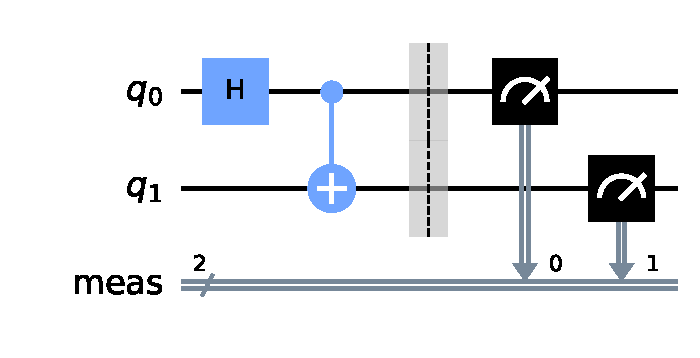
\includegraphics[scale=0.5]{epr_pair}
    \caption{Створення стану Белла $\ket{\Phi^+}$}
    \label{epr_circuit}
\end{figure}
Розглянемо приклад схеми зображеної на Рис. \ref{epr_circuit}. 
На схемі кожен кубіт зображений горизонтальною лінією, а усі  вентилі розташовані на лініях тих кубутів, над якими відбувається дія. 
Ця схема є результатом виконання наступного коду:
\begin{lstlisting}[language=Python]
    circuit = QuantumCircuit(2)
    circuit.h(0)
    circuit.cnot(0, 1)
    circuit.measure_all()
    circuit.draw('mpl', filename="epr_pair.pdf")
\end{lstlisting}

При створені схеми, вихідне значення кожного кубіта дорівнює $\ket{0}$, отже початковий стан системи можна писати наступним рівнянням: $\ket{\psi} = \ket{00}$. 

Далі до першого кубіта застосовується перетворення Адамара. Вентиль який утилізує це перетворення позначається літерою $H$\footnote{Від англійського Hadamard gate} та може бути представленим у вигляді матриці наступним чином:
\begin{align}
H=\frac{1}{\sqrt{2}}
\begin{bmatrix} 
    1 & 1\\1 & -1
\end{bmatrix}
\label{hadamard}
\end{align}

Після дії перетворення Адамара, стан системи описується наступним рівнянням: $\ket{\psi} =\frac{1}{\sqrt{2}} (\ket{00}+\ket{10})$.

Наступним є вентиль $CNOT$ -- контрольоване заперечення. 
Якщо контрольний кубіт має значення $\ket{0}$ жодної дії не відбудеться, проте, якщо він має значення $\ket{1}$, значення цільового кубіта перевернеться.
Більш формально дію цього оператора можна описати наступною матрицею:
$$
CNOT = \begin{bmatrix}
    1 & 0 & 0 & 0 \\
    0 & 1 & 0 & 0 \\
    0 & 0 & 0 & 1 \\
    0 & 0 & 1 & 0
\end{bmatrix}
$$

Таким чином після дії цього вентиля на $q_1$ з контрольним кубітом $q_0$ стан системи можна описати наступним рівнянням: $\ket{\psi} =\frac{1}{\sqrt{2}} (\ket{00}+\ket{11})$, що є одним з станів Белла -- $\ket{\Phi^+}$.

Останнім елементом цієї схеми є вимір. 
Вимір у квантовому світі -- це проєктування стану в якому перебуває кубіт на один з базисних векторів. 
Для квантових комп'ютерів базисними є вектори $\ket{0}$ та $\ket{1}$, таким чином після виміру $q_0$ уся система сколапсує в один з двох станів $\ket{\psi_0}=\ket{00}$, або $\ket{\psi_1}=\ket{11}$, а отже, результат виміру $q_1$ вже однозначно визначений.

\subsubsection{Запуск схем}

Подивитися на те, що ж насправді робить складена схема можна запустивши її на симуляторі. 
Це можна зробити наступним чином:

\begin{lstlisting}[language=Python]
    simulator = Aer.get_backend('aer_simulator')
    circ = transpile(circuit, simulator)
    counts = simulator.run(circ).result().get_counts()

    plot_histogram(counts)
\end{lstlisting}

Результатом буде гістограма, схожа на зображену на Рис. \ref{simulator_results} \footnote{Точні значення можуть і будуть відрізнятися, оскільки колапс $q_0$ -- випадковий процес}.

\begin{figure}[bh]
    \centering
    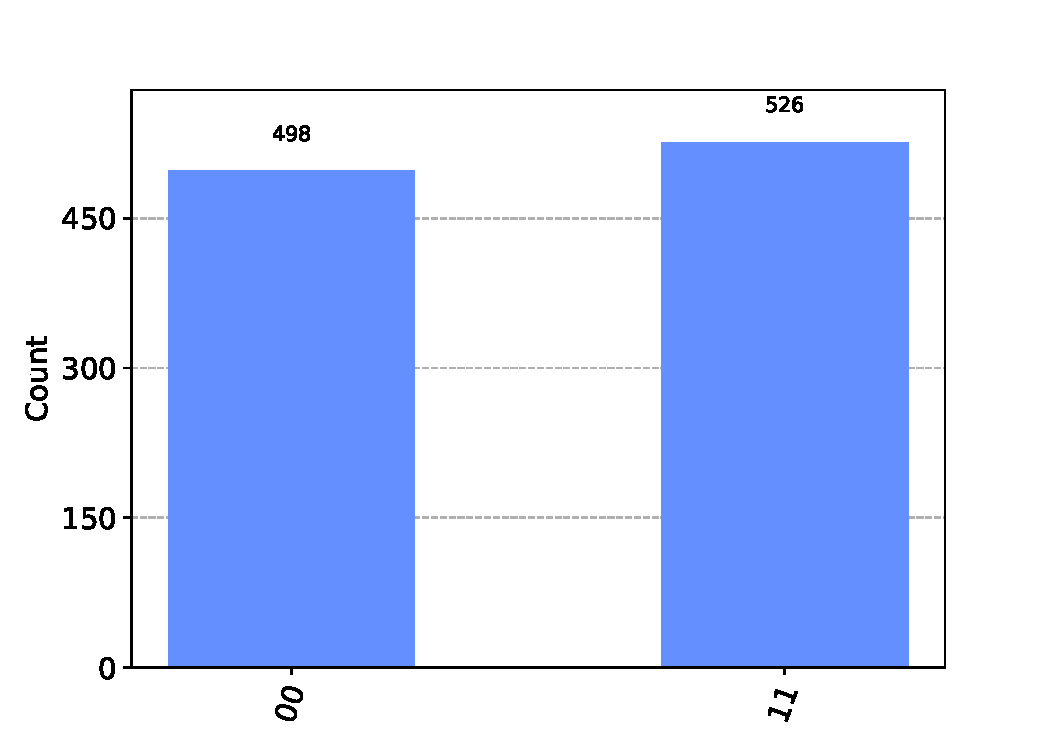
\includegraphics[scale=0.3]{results}
    \caption{Результат запуску схеми на симуляторі}
    \label{simulator_results}
\end{figure}

Після того як ми запустили нашу схему на симуляторі та пересвідчиилися в правильності резільтатів можна спробувати запустити цю схему на справжньому квантоваму комп'ютері компанії IBM.

Для цього перш за все необхідно отримати свій особистий ключ від IBM Quantum. 
При наявності свого токену, запуск на квантовому комп'ютері не сильно відрізняється від запуску схеми на симуляторі: 
\begin{lstlisting}[language=Python]
    provider = IBMProvider(token="IBM_QUANTUM_TOKEN")
    backend = provider.get_backend("ibm_nairobi")
    
    transpiled_circuit = transpile(circuit, backend)
    job = backend.run(transpiled_bv_circuit)
    print(job.job_id())

    counts = job.result().get_counts()
    plot_histogram(counts)
\end{lstlisting}

\subsubsection{Корисні вентилі}

Перерахую тут усі поширені вентилі які можливо можуть можуть знадобитися:
\begin{itemize}
    \item \href{https://qiskit.org/documentation/stubs/qiskit.circuit.library.HGate.html#hgate}{HGate} -- перетворення Адамара (\ref{hadamard}). Також може бути додана до схеми за допомогою метода $h(targets)$ ($ch(controls, targets)$).
    \item \href{https://qiskit.org/documentation/stubs/qiskit.circuit.library.XGate.html#xgate}{XGate} -- перетворення, яке відповідає матриці Паулі $\sigma_x$ (\ref{sigmax}). Також може бути додана до схеми за допомогою метода $x(targets)$ ($cx(controls, targets)$, або синонім $cnot(controls, targets)$).
    \item \href{https://qiskit.org/documentation/stubs/qiskit.circuit.library.YGate.html#ygate}{YGate} -- перетворення, яке відповідає матриці Паулі $\sigma_y$ (\ref{sigmay}). Також може бути додана до схеми за допомогою метода $y(targets)$ ($cy(controls, targets)$).
    \item \href{https://qiskit.org/documentation/stubs/qiskit.circuit.library.ZGate.html#zgate}{ZGate} -- перетворення, яке відповідає матриці Паулі $\sigma_z$ (\ref{sigmaz}). Також може бути додана до схеми за допомогою метода $z(targets)$ ($cz(controls, targets)$).
\end{itemize}

\subsubsection{Проєктування не на стандартний базис}

Як я вже казав раніше, вимір -- проєктування на базис. У випадку квантових комп'ютерів, проєктування завжди відбувається на стандартний базис, а отже проведення більш складних вимірів\footnote{Таких як виміри Белла, наприклад} необхідні додаткові дії.

Для проведення такого виміру, необхідно знайти оператор, який переводить базис на який необхіднно зробити проєкцію у стандартний бази, на який вміє проєктувати квантовий комп'ютер.
Таким чином для проведення вимірів Белла, необхідно знайти схему яка перетворить стани Белла $\ket{\Phi^+}$, $\ket{\Psi^+}$, $\ket{\Phi^-}$ та $\ket{\Psi^-}$ на стандартний базис $\ket{00}$, $\ket{01}$, $\ket{10}$ та $\ket{11}$ відповідно.

На Рис. \ref{epr_circuit} ми використовуючи два вентилі перетворили стан $\ket{00}$ у стан $\ket{\Phi^+}$. Неважко переконатися, що та ж схема перетворює інші вектори стандартного базису на відповідні стани Белла:

\begin{align*}
\ket{01} \xRightarrow{H} \frac{1}{\sqrt{2}} (\ket{01}+\ket{11}) \xRightarrow{CNOT} \frac{1}{\sqrt{2}} (\ket{01}+\ket{10}) = \ket{\Psi^+} \\
\ket{10} \xRightarrow{H} \frac{1}{\sqrt{2}} (\ket{00}-\ket{10}) \xRightarrow{CNOT} \frac{1}{\sqrt{2}} (\ket{01}-\ket{11}) = \ket{\Phi^-} \\
\ket{11} \xRightarrow{H} \frac{1}{\sqrt{2}} (\ket{01}-\ket{11}) \xRightarrow{CNOT} \frac{1}{\sqrt{2}} (\ket{01}-\ket{10}) = \ket{\Psi^-}
\end{align*}

Якщо ж застосувати ці ж вентилі, але у звооротньому порядку на стани Белла, тоді вони перетворяться на вектори стандартного базису, а отже подіявши цими двома вентилями на стан (\ref{bell_state}) ми отримаємо наступний стан:
\begin{align*}
    \ket{\psi_0} \xRightarrow{CNOT, H} \ket{\psi_1} = \frac{1}{2}\big[
    \ket{00}_{\psi A}(\alpha\ket{0}_B + \beta\ket{1}_B) + \\
    \ket{10}_{\psi A}(\alpha\ket{0}_B - \beta\ket{1}_B) + \\
    \ket{01}_{\psi A}(\alpha\ket{1}_B + \beta\ket{0}_B) + \\
    \ket{11}_{\psi A}(\alpha\ket{1}_B - \beta\ket{0}_B)
    \big]
\end{align*}

Цей стан виражений у стандартному базисі, а отже після виміру на квантовому комп'ютері система сколапсує в один з цих доданків.

\end{document}
